\documentclass[12pt, twoside]{article}
\usepackage[left=2.5cm,right=2cm,top=2cm,bottom=2cm]{geometry}

\usepackage{lastpage}
\usepackage{fancyhdr}
\pagestyle{fancy}
\renewcommand{\headrulewidth}{0.4pt}
\renewcommand{\footrulewidth}{0.4pt}
\renewcommand{\sectionmark}[1]{ \markright{#1}{} }
\lhead{Cyril NOVEL}\chead{Rapport de stage}\rhead{\textit{ \nouppercase{\rightmark}}}
\lfoot{}\cfoot{\thepage\ / \pageref{LastPage}}\rfoot{}

\setlength{\headheight}{15pt}

\usepackage[french]{babel}
\usepackage[utf8]{inputenc}
\usepackage{amsmath}
\usepackage{graphicx}
%\usepackage{algpseudocode}
\usepackage{algorithm}
\usepackage{amsthm}
\usepackage{amssymb}
\usepackage{mathtools}
\usepackage{commath}
\usepackage{stmaryrd}
\usepackage{url}
\usepackage{caption}
\usepackage{subcaption}
\usepackage{hyperref}
\usepackage[noend]{algpseudocode}
\usepackage{listings}
\usepackage[usenames,dvipsnames,svgnames,table]{xcolor} % for setting colors
\usepackage{courier}

\let\oldsection\section
\def\section{\cleardoublepage\oldsection}

\renewcommand*\lstlistingname{Code}
% set the default code style
\lstset{
    frame=tb, % draw a frame at the top and bottom of the code block
    tabsize=2, % tab space width
    showstringspaces=false, % don't mark spaces in strings
    numbers=left, % display line numbers on the left
    commentstyle=\color{gray}, % comment color
    keywordstyle=\color{blue}, % keyword color
    stringstyle=\color{red}, % string color
    basicstyle=\footnotesize\ttfamily
}

\hypersetup{
  colorlinks=true,
  citecolor=black,
  urlcolor=Cerulean,
  linkcolor=PineGreen,
}

\title{Stage de fin d'études\\
\large{École polytechnique - Acute3D}}

\author{Cyril NOVEL}

\date{\today}

\begin{document}

\begin{titlepage}
\begin{center}

\includegraphics[width=0.20\textwidth]{LogoX.jpg}~\\[0.5cm]

\includegraphics[height=0.12\textwidth]{LogoA3D.jpg}~\\[1cm]

\textsc{\LARGE École polytechnique}\\[0.5cm]

\textsc{\Large Département d'informatique}\\[1.5cm]

% Title
\rule{\textwidth}{.4pt}
{ \huge \bfseries Sémantisation géométrique de modèles de villes : détection de plans \\[0.4cm] }

\rule{\textwidth}{.4pt}\\[1.5cm]

% Author and supervisor
\begin{minipage}{0.4\textwidth}
\begin{flushleft} \large
\emph{Auteur:}\\
Cyril \textsc{Novel}
\end{flushleft}
\end{minipage}
\begin{minipage}{0.4\textwidth}
\begin{flushright} \large
\emph{Superviseur:} \\
Renaud \textsc{Keriven}
\end{flushright}
\end{minipage}

\vfill
{\large \today}
\end{center}
\end{titlepage}

\newpage
\begin{abstract}
Dans ce rapport,

nous proposons ensuite de sémantiser à l'aide de plans

2 OK

pour ce type d'application et pas genre

\end{abstract}~\\[5cm]
\addcontentsline{toc}{section}{Résumé}

\section*{Remerciements}
\addcontentsline{toc}{section}{Remerciements}
Je voudrais remercier mon superviseur Renaud Keriven, qui a su dirigé mes efforts, ainsi que Jean-Phillipe Pons. Je remercie aussi toute l'équipe d'Acute3D qui m'a réservé un accueil chaleureux et m'a permi de travailler dans un excellent environement.
\newpage

\tableofcontents
\newpage

\section*{Introduction}
\addcontentsline{toc}{section}{Introduction}
La création de modèles tridimensionnels de villes à partir de données photographiques ou de relevés lasers de manière automatique est en plein essor. De nombreux acteurs, tels Google, Apple ou Microsoft, proposent de visualiser des villes et des bâtiments en trois dimensions avec leur logiciels de cartographie respectifs. Les problèmes soulevés sont nombreux. L'objectif initial consistant à obtenir un modèle précis et détaillé a été longuement étudié et de nombreuses techniques permettent d'obtenir des résultats satisfaisants.

De nos jours, la diffusion de ces modèles se fait via l'Internet, voire via les réseaux mobiles sur smartphones et tablettes. La vitesse de connexion peut fortement varier selon les casd'utilisation. Il est alors crucial de réduire le poids du modèle créé tout en maintenant un niveau de détail suffisant, afin de permettre un téléchargement plus rapide du modèle. Il est nécessaire de simplifier intelligemment le modèle, en prenant en compte la géométrie et la topologie de la reconstruction. On parle alors de sémantisation du modèle.

Avant de repérer des structures complexes, comme les types de bâtiments ou les détails architecturaux, la première étape consiste à identifier des primitives géométriques -- plans, cylindres, quadriques -- pour simplifier le modèle. Si des travaux existent à ce sujet, ils ne prennent pas en compte les spécificités des modèles 3D de villes, comme le manque de précision et le bruit ainsi que la variation de l'échantillonage au sein du modèle. La détection de plans va permettre de réduire le poids du modèle.

L'objectif de ce stage est de développer un algorithme capable de détecter des plans dans un modèle 3D. Cette détection doit pouvoir s'adapter de manière automatique au modèle traité, que ce soit au niveau du bruit, de la précision ou de l'échelle. Il est aussi nécessaire que cette détection puisse être paramétrée, c'est à dire que l'utilisateur puisse définir une tolérance d'erreur pour les plans. L'algorithme doit ensuite créer les plans tout en conservant la topologie du modèle. Une étape de simplification est ensuite nécessaire pour réduire la taille du modèle obtenu. Cette étape de simplification doit prendre en compte la présence des plans afin de ne pas déformer ces derniers.
\newpage

\section{Détection de plans}
\subsection{Problématique}
Détecter des plans est la première étape de notre algorithme global. Avant tout, il a fallu choisir l'objet qui allait être traité. Le logiciel \textit{Smart3DCapture} génère plusieurs objets tout au long de la chaîne de traitement. Un nuage de points bruité est généré, suivi par un maillage 3D grossier et ensuite d'un maillage 3D précis. Il aurait été possible d'extraire des plans du nuage bruité. Cependant des détails -- fenêtres, cheminées -- auraient êté confondus avec un plan. Il a donc été décidé d'extraire des plans à partir du maillage 3D précis.

Le maillage possède aussi un avantage certain sur le nuage de points. De nombreuses informations sont plus simples et plus rapides à calculer grâce à la connectivité du maillage. L'estimation de l'échantillonage devient triviale, de même que l'estimation de la normale.

Par la suite, nous détaillons les algorithmes les plus courants pour extraire des plans d'un nuage de points ou d'un maillage. Nous aborderons l'algorithme \textit{RANSAC}, la transformée de Hough et la croissance de région.

\subsection{RANSAC}
Le \textit{RANSAC} -- \textit{RANdom SAmple Consensus} -- est un algorithme itératif non déterministe. Soit un nuage de points $C$. À chaque itération de l’algorithme, on choisit un nombre $p$ de points au sein du nuage de points de manière aléatoire. On note $S$ cet ensemble. On calcule alors le meilleur plan pour cet ensemble de points, c’est à dire le plan qui minimise la somme des distances au carré de points à ce plan -- cf annexe. Une fois le plan trouvé, on parcourt les points de $C\setminus S$. Si le point correspond au plan avec une certaine erreur $d$, on l’ajoute à l’ensemble $S$. Une fois l’ensemble des points de $C\setminus S$ parcouru, on recalcule le meilleur plan pour l’ensemble $S$. Si le plan est meilleur que celui de l’itération précédente -- la somme des distances au carré est plus faible, alors on le considère comme le meilleur plan courant. Sinon le plan de l’itération précédente reste le meilleur plan courant. On procède ainsi pendant $k$ itérations, $k$ étant fixé à l’avance. Une fois le meilleur plan trouvé, $C$ = $C\setminus S$ et on effectue un nouveau \textit{RANSAC} sur $C$ pour trouver le prochain plan. Il est possible de s’arrêter avant la $k$ème itération si une itération est suffisamment bonne, c’est à dire que l’erreur est suffisamment faible.

\textit{RANSAC} a l’avantage de posséder une excellente robustesse aux outliers \cite{RANSAC1}. Cependant, l’algorithme est lent. Pour les $k$ itérations, on ne trouve qu’un seul plan. Il faut donc répéter la méthode $n$ fois pour trouver $n$ plans. Le nombre de plans est totalement dépendant de la scène considérée, il est difficile d’estimer ce paramètre correctement. Une solution peut être de fixer une erreur minimale maximale. Si au $i^\text{ème}$ plan, à la $k^\text{ème}$ itération, l’erreur minimale est supérieure à un certain seuil, alors on arrête la recherche. Une autre amélioration consiste à sélectionner les points dans un certain voisinage, afin d’augmenter la probabilité de détecter un plan.

Un autre problème réside dans la taille variable des plans. Dans un modèle de ville, les rues sont planes tout comme certains toits. Les rues contiennent plus de 50000 points alors qu'un pan de toit va contenir moins de 700 points. Le choix de la variable $p$ est difficile. Il faudrait l'initialiser à moins de 700 points pour espérer obtenir le pan de toit. Sachant que le nuage peut contenir plus de 2 millions de points, le temps d'exécution du \textit{RANSAC} devient extrêmement long.

Afin de raccourcir le temps d'exécution, il est possible de segmenter le nuage de points en une grille 3D, comme proposé par \cite{RANSAC2}. Pour chaque bloc un algorithme de \textit{RANSAC} est lancé. Facilement parallélisable, cette technique a aussi l'avantage d'être moins coûteuse -- moins de points à tester. Le choix de la variable $p$ est moins compliqué puisque la taille des plans est limité par la taille des cases. Cependant, la segmentation crée d'autres problèmes. Si un plan présent dans une case $C_1$ déborde légèrement dans une case $C_2$, il ne sera pas détecté dans cette dernière. La détection des plans n'est donc pas optimale. D'autre part, chaque plan est segmenté sur chaque case. Si un plan traverse $n$ cases, il y aura $n$ équations différentes pour ce plan. Une étape supplémentaire de fusion doit donc être considérée pour obtenir un résultat acceptable.

L'ensemble de ces éléments ne permet pas de retenir \textit{RANSAC} pour notre problématique.

\subsection{Transformée de Hough}
La transformée de Hough est une méthode qui permet de détecter des objets paramétrés, des plans dans notre cas. L’idée est de transformer un point $p$ de l’espace euclidien 3D en une courbe dans l’espace de Hough. Cette courbe représente l’infinité des plans passant par $p$. D’un point $p = (p_x; p_y; p_z)$, on donne l’équation d’un plan passant par $p$ selon trois variables qui sont la distance à l’origine $\rho$, l’angle $\theta$ de la normale du plan sur le plan $xy$ et l’angle $\phi$ entre le plan $xy$ et la composante selon $z$ de la normale -- Fig~\ref{fig:Hough1}. L’équation suivante régit la relation entre $p$ et ($\rho, \theta, \phi$) :
$$p_x*cos\theta * sin\phi + p_y*sin\theta*sin\phi + p_z*cos\phi = \rho$$
Dans l'espace de Hough, chaque triplet ($\rho, \theta, \phi$) décrit un unique plan de $\mathbb{R}^3$.

\begin{figure}[h]
\centering
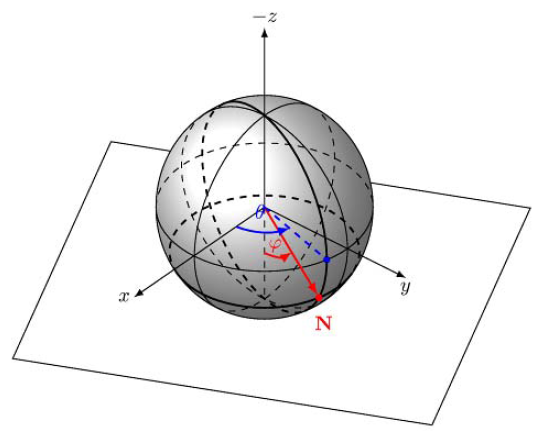
\includegraphics[scale=0.5]{HoughCoord.png}
\caption{\label{fig:Hough1} Coordonnées ($\rho, \theta, \phi$)}
\end{figure}

Afin de trouver les plans d’un nuage de points, on calcule la transformée de Hough pour chaque point $p$, c’est à dire l’ensemble des triplets ($\rho, \theta, \phi$) vérifiant l’équation ci-dessus. L’ensemble de ces points forme une sinusoïde dans l’espace de Hough. On trouve les plans lorsque 3 courbes ou plus s’intersectent au même triplet dans l’espace de Hough -- Fig~\ref{fig:Hough2}. Ainsi, pour un nuage de points donné, plus il y a de courbes qui s’intersectent au même point ($\rho, \theta, \phi$), plus la probabilité que le plan associé soit un plan recherché est forte.

\begin{figure}[h]
\centering
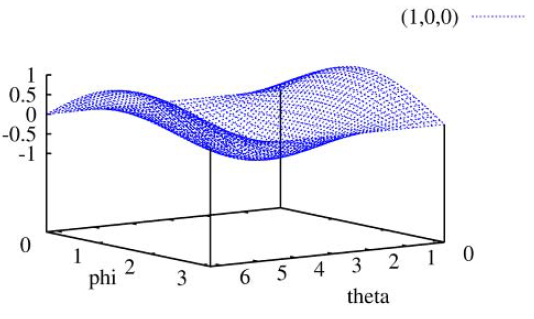
\includegraphics[scale=0.5]{HoughCurv1.png}~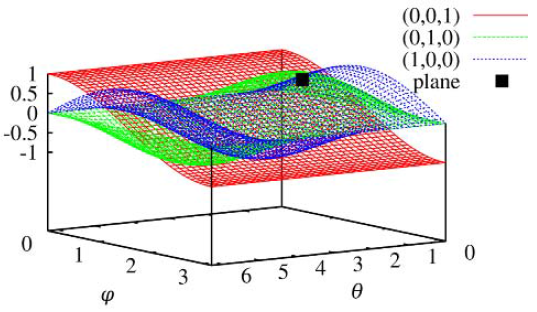
\includegraphics[scale=0.5]{HoughCurv0.png}
\caption{\label{fig:Hough2} À gauche, la courbe formée par un point de l’espace XYZ. À droite, l’intersection de trois courbes définit un plan.}
\end{figure}

Dans \cite{Hough1}, plusieurs méthodes sont décrites pour effectuer cette recherche de plans. Nous ne détaillons ici que la méthode la plus basique, appelée \textit{Transformée de Hough Standard} -- \textit{Standard Hough Transform}. Dans cette méthode, l'espace de Hough est discrétisé en différentes cellules. Chaque cellule contient un score. Pour chaque point $p$ du nuage de points, on incrémente les cellules touchées par la transformée de Hough associée, c'est à dire les cellules où la courbe passe effectivement. Après traitement du nuage de points en entier, les cellules avec les scores les plus grands représentent les plans du nuage de points.

Selon la taille choisie pour les cellules et le bruit présent dans le nuage de points, un mécanisme de cellule cubique volante peut être mis en place pour rechercher les meilleurs plans. Ces derniers correspondent au centre de la cellule volante lorsque le score dépasse un certain seuil $T$.

La Transformée de Hough Standard est un algorithme lent. La complexité de l'incrémentation est $O(n*N_{\theta}*N_{\phi})$ où $n$ est le nombre de points, $N_{\theta}$ le nombre de cellules selon $\theta$ et $N_{\phi}$ le nombre de cellules selon $\phi$. Dans \cite{Hough1}, un nuage de 60000 points est traité en 6 minutes. Pour un modèle de villes de l'ordre de 2 millions de points, le temps de traitement passe à plus de 3 heures. D'autres méthodes sont plus rapides, mais deviennent inexactes.

Au lieu d'utiliser les points, il est possible dans notre cas d'utiliser les facettes du maillage. En effet chaque facette $f$ correspond à un plan. $f$ peut être projetée dans l'espace de Hough en trouvant directement ses coordonnées ($\rho, \theta, \phi$). Ainsi, au lieu de créer une courbe et de tester l'intersection avec l'ensemble des cellules possibles, il est désormais possible de voter directement pour la cellule correspondante. Cela réduit largement la complexité de l'algorithme de vote : la compléxité devient $O(N_f)$ où $N_f$ est le nombre de facettes dans le maillage. Sachant que dans les modèles que nous traitons, nous constatons empiriquement que $N_f ~ 2n$, la complexité de cette méthode est effectivement plus faible que celle de la Transformée de Hough Standard.

Quelle que soit la variante de la transformée de Hough utilisée, il est nécessaire de discrétiser l'espace de Hough. Cette discrétisation, ou design de l'accumulateur, est importante. En effet, un mauvais accumulateur peut entraîner plusieurs problèmes :
\begin{itemize}
  \item échec dans la détection des plans ;
  \item lenteur ;
  \item mauvaise précision ;
  \item taille des données importantes.
\end{itemize}
La principale difficulté dans le design de l'accumulateur se trouve dans la discrétisation des angles $\theta$ et $\phi$, afin d'obtenir des zones de tailles égales sur la sphère unité. Par la suite, nous allons présenter les différentes discrétisations possibles, en détaillant les trois accumulateurs les plus classiques décrits dans \cite{Hough2}.

\paragraph{Tableau}
L’accumulateur de type Tableau -- Fig~\ref{fig:Array} -- est simple à définir. Deux pas sont choisis pour chaque variable -- $\Delta_{\theta}$ et $\Delta_{\phi}$, et les cellules sont définies selon ces pas. Une telle discrétisation possède un désavantage certain. La taille des cellules n’est pas constante et peut fortement varier d’une cellule à l’autre.

\begin{figure}[h]
\centering
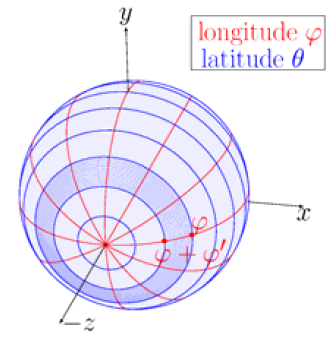
\includegraphics[scale=0.65]{Array.png}
\caption{\label{fig:Array} L'accumulateur de type Tableau}
\end{figure}

On constate que le score des cellules équatoriales sera plus élevé que celui des cellules polaires, la détection des plans sera donc faussée. Il est d’une part difficile de choisir un bon seuil de détection, et des plans différents risquent de voter pour la même cellule. L’approche Tableau est trop simpliste pour être satisfaisante.

\paragraph{Cube}
L’accumulateur de type Cube -- Fig~\ref{fig:Cube} -- cherche à compenser ce problème de taille des cellules, tout en restant simple à implémenter. L’idée est qu’une correspondance entre les cellules de l’accumulateur et des petits patchs sur la sphère unité doit exister. La solution est de projeter la sphère unité sur le plus petit cube aligné sur la base contenant la sphère à l’aide du difféomorphisme
$$\varphi \text{: } S^2 \rightarrow cube$$
$$s \mapsto s/\lVert s\rVert_{\infty}$$
Chaque face du cube est ensuite divisée en une grille régulière. Étant donné la normale $n$ d’un plan, on retrouve la cellule dont le score doit être augmenté de la façon suivante. Le côté $a_i$ du cube est déterminé par la direction dominante $n_d$. La projection sur ce cube se fait en multipliant $n$ par $n_d$. Les coordonnées non dominantes deviennent alors $c_x =
\dfrac{n_1}{n_d}$ et $c_y = \dfrac{n_2}{n_d}$ -- $n_1$ et $n_2$ représentent les deux directions non dominantes de $n$. On calcule alors les coordonnées de la cellule comme suit :

\begin{equation*}
  a_x = 
     \begin{cases}
        1 & \text{si $\dfrac{c_x + 1}{2} = 1$} \\
        1 + nr_cells*\dfrac{c_x + 1}{2} & \text{sinon}
     \end{cases}
\end{equation*}

\begin{equation*}
  a_y = 
     \begin{cases}
        1 & \text{si $\dfrac{c_y + 1}{2} = 1$} \\
        1 + nr_cells*\dfrac{c_y + 1}{2} & \text{sinon}
     \end{cases}
\end{equation*}

\begin{figure}[h]
\centering
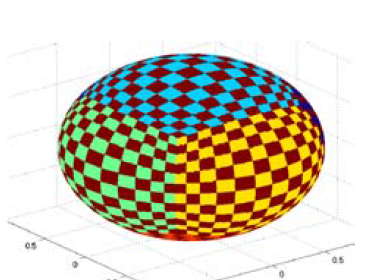
\includegraphics[scale=0.65]{Cube.png}
\caption{\label{fig:Cube} L'accumulateur de type Cube}
\end{figure}

La relation entre l’accumulateur et $S$ est donc simple. La Fig 1.4 montre que les patchs sur la sphère sont plus réguliers que pour l’accumulateur Tableau. L’accumulateur Cube est aussi invariant par une rotation de 90 degrés autour des axes du repère. Cependant, les cellules sont quand même plus petites sur les arêtes du cube qu’au centre des faces. L’accumulateur aura donc plus de mal à détecter un plan si sa normale pointe en direction d’un coin de l’accumulateur Cube. Par ailleurs, l’accumulateur est aussi sensible aux rotations d’angle de moins de 90 degrés.

\paragraph{Balle}
L’accumulateur de type Balle -- Fig~\ref{fig:Ball} -- cherche à discrétiser l’espace de Hough en cellules de taille égale, afin de pallier aux problèmes évoqués. Pour cela, la résolution des patchs doit être différente selon la position sur la sphère unité. La résolution selon $\phi$ est semblable à celle de l’accumulateur Tableau, c’est à dire à pas constant $\Delta_{\phi}$. Selon l’angle $\phi$, l’angle $\theta$ va évoluer de manière à ce que les cellules gardent une taille constante. Le cercle de diamètre le plus grand est situé à l’équateur -- soit $\phi = 0$. Pour la sphère unité, son périmètre est $max_l = 2\pi$. Pour le cercle situé à l’angle $\phi$, la longueur est $l_i = 2\pi \phi$. Ainsi
$$\Delta_{\theta} = \dfrac{360*max_l}{l_i*N_{\theta}}$$
où $N_{\theta}$ est la résolution souhaitée. L’accumulateur obtenu est bien constitué de cellules de taille égale. Par contre, l’invariance par rotation de 90 degrés n’est pas conservée. Cette difficulté peut être contournée en choisissant une résolution fine pour la phase de vote et une détection avec une cellule volante.

\begin{figure}[h]
\centering
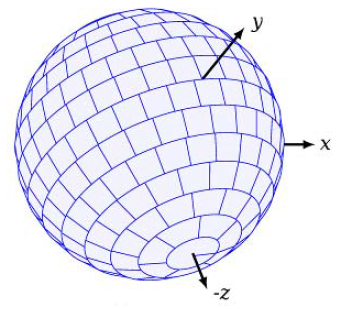
\includegraphics[scale=0.65]{Ball.png}
\caption{\label{fig:Ball} L'accumulateur de type Balle}
\end{figure}

Notre objectif est de traiter des maillages très grands -- 2 millions de points et 4 millions de facettes. Il est donc nécessaire que l'accumulateur soit assez détaillé pour ne pas confondre plusieurs plans.

XXX

le plus propice -> le plus efficient pour détecter les plans.

à finir...

\subsection{Croissance de région}
La croissance de région -- \textit{region growing} -– est une approche gloutonne de la détection de plan. L’idée de base est de partir d’un point graine et d’ajouter tous ses proches voisins, tant que ces voisins respectent l’équation du plan initial. Une méthode basique est présentée dans \cite{reggrow1}. On choisit 3 points du nuage de points qui se trouvent dans une sphère de rayon $r$. Ces trois plans initialisent le plan optimal $\Pi$ et le set de points $S$. Ensuite, on cherche le point $p$ tel que
\begin{itemize}
  \item $p$ est le plus proche voison de $S$ ;
  \item $\text{dist}(S,p) < \delta$ ;
  \item $\text{dist}(S,p) < \gamma$ ;
  \item l'erreur entre $S\cup\{p\}$ et $\Pi$ est inférieure à $\epsilon$.
\end{itemize}

L'expansion de la région s'arrête lorsqu'il n'est plus possible de trouver de nouveaux points à insérer. On vérifie alors que $\vert S\vert < \Theta$, c'est à dire que la région est suffisamment grande pour être jugée intéressante. Ensuite, les points sont retirés du nuage de points initial et une nouvelle phase de croissance de plan commence. Le plan optimal est obtenu grâce à la méthode détaillée en annexe.

La principale difficulté de la croissance de région est de sélectionner correctement les trois points de départ. En effet, il serait intéressant d'écarter mes zones ne correspondant pas à des plans. Sur ce type de zones, l'algorithme va lancer plusieurs fois la croissance de région, pour des régions qui seront très petites. Du temps peut être gagné en affinant la sélection des trois premiers points.

\cite{reggrow2} propose une technique pour choisir de manière plus efficace le point de départ de la croissance de région. On cherche un point de départ $p_s$ qui vérifie les deux critères suivants :
\begin{itemize}
  \item $p_s$ a au moins 6 voisins, c'est à dire la sphère de centre $p_s$ et de rayon $\delta$ contien au moins 6 points ;
  \item le voisinage de $p_s$ est localement plan, c'est à dire que les points contenus dans la sphère précédente forment un plan.
\end{itemize}
Le premier critère assure que la région est suffisamment peuplée, et qu’une recherche dans ce voisinage est intéressante. Le second critère assure un semblant de plan. Il évite de débuter une séquence de croissance alors qu’il n’y a que peu de chance que la région considérée soit un plan. On estime la planarité du voisinage de la même manière que précédemment.

Une autre méthode est décrite dans \cite{reggrow3} pour trouver des plans via la croissance de régions. Il s'agit dans un premier temps de calculer la normale de chaque point ainsi que la courbure à chaque point. Ces deux variables sont obtenues via une \textit{Principal Components Analysis} décrite en annexe. Les points sont ensuite filtrés selon leur courbure $\gamma$ : si $\gamma < S_c$, alors le point est considéré comme graine. Les graines sont classées par ordre croissant de courbure. Ensuite les graines sont réparties sur la sphère unité selon leur normale. Une étape de clustering est ensuite appliquée :
\begin{itemize}
  \item La graine avec la courbure la plus faible $g$ est choisie et le cluster $C$ est initialisé avec $g$ ;
  \item On ajoute au cluster $C$ les points $p$ tel que $n_p\cdot n_g \approx 1$ et tel que $\text{max}\{n_p\cdot(p-g), n_g\cdot(p-g)\}$ est proche de 0 -- c'est-à-dire $p-q$ orthogonal à la normal du plan ;
  \item Une fois qu'on ne peut plus ajouter de points, si $\vert C\vert > T$ un seuil alors le cluster est validé et les points sont retirés du nuage de points. Sinon $g$ est retiré de la liste des graines.
\end{itemize}
Cet algorithme est répété jusqu'à ce que la liste des graines soit vide. La particularité de cette croissance de région est qu'elle s'opére sur la sphère unité et non pas sur le nuage de points. La figure~\ref{fig:GaussMap} illustre cet algorithme.

\begin{figure}[h]
\centering
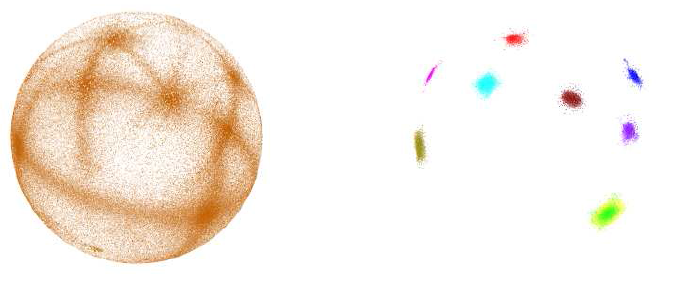
\includegraphics[scale=0.65]{GaussMap.png}
\caption{\label{fig:GaussMap} À gauche, la répartition des graines sur la sphère unité. À droite les clusters obtenus.}
\end{figure}

Notre méthode propose un mélange dans les techniques de croissance de régions. Nous commençons par évaluer la courbure de chaque facette via la méthode de \cite{reggrow3}. Grâce au maillage, le voisinage de la facette s'obtient facilement. Il suffit de prendre les $n$ premières couronnes de points autour de la facette -- Fig \ref{fig:couronne}.

\begin{figure}[h]
\centering
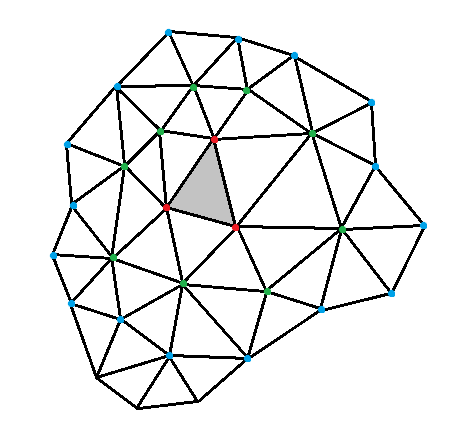
\includegraphics[scale=0.5]{Couronnes.png}
\caption{\label{fig:couronne} Couronnes successive d'un triangle. En rouge, la première couronne, en vert la seconde, en bleu la troisième.}
\end{figure}

Si la courbure de la facette est inférieure à un seuil, la facette est ajoutée dans la liste des graines. Lorsque toutes les facettes sont traitées, on classe la liste par ordre croissant de courbures. La graine la plus probable -- car se trouvant à l'endroit le plus plan -- se trouve donc en début de liste.

Chaque facette est ensuite traitée dans une phase de croissance de région. L'algorithme suivant est appliqué :
\begin{enumerate}
  \item On sélectionne la facette $f$, le premier élément de la liste des graines. On crée l'ensemble $P$ le plan que l'on cherche et $f$ est ajoutée à $P$ ;
  \item On ajoute les 3 voisines de $f$ à la queue $Q$ ;
  \item On sélectionne le premier élément de $Q$. Si cette facette est cohérente avec le plan, elle est ajoutée à $P$ et ces trois voisines sont ajoutées à $Q$ -- sauf si elles ont déjà été ajoutées ;
  \item On itère l'étape précédente jusqu'à ce que $Q$ soit vide ;
  \item On vérifie que le plan $P$ est effectivement un plan ;
  \item On retire les facettes de $P$ de la liste des facettes à traiter.
\end{enumerate}

Les critères de cohérence de facette et de calcul du plan sont détaillés dans la partie~\ref{subsec:growthimpl}. Notre algorithme de croissance de région est rapide. L'information de courbure est obtenu rapidement grâce au maillage et le traitement de chaque facette peut se faire en parallèle. À l'inverse d'un \textit{RANSAC} ou de la transformée de Hough, la croissance de région permet d'obtenir une information locale sur le plan : les facettes qui constituent le plan forment une unique composante. L'utilisation de graines permet de choisir correctement le plan de départ et de traiter d'abord les plans les plus probables. Enfin, l'intérêt de l'utilisation d'un maillage par rapport au nuage des point réside dans l'attribution des plans à des facettes et non pas à des points. En effet, un point peut appartenir à plusieurs plans -- s'il se trouve sur une arête ou dans un coin par exemple -- mais une facette ne peut appartenir qu'à un seul plan. L'utilisation des facettes permet de lever facilement l'ambiguïté existante dans un nuage de points.

\subsection{Implémentation}
\label{subsec:growthimpl}
L'implémentation de notre algorithme a été réalisée en \texttt{C++} et avec \texttt{OpenMP} pour la parallélisation.

La première partie de l'algorithme réside dans le calcul des informations de chaque facette. Durant cette phase, 3 valeurs sont calculées et attribuées à la facette : la normale, la normale étendue et la courbure. La normale est calculée simplement grâce à un produit vectoriel entre deux côtés de la facette. Le calcul de la courbure et de la normale étendue est détaillé en annexe. La principale difficulté de cette étape se trouve dans le parcours des points autour de la facette. Nous avons mis en place la méthode par récurrence suivante :
\begin{itemize}
  \item La première couronne est constituée des 3 points de la facette ;
  \item Sachant que nous avons obtenu toutes les couronnes de $1$ à $n-1$, la couronne $n$ est composée des sommets adjacents à la couronne $n-1$ non encore visité.
\end{itemize}
Cette méthode tire profit de la technique de parcours sur un \textit{mesh}. Il est facile de parcourir les voisins d'un sommet en étoilant autour de ce dernier.

La taille de la couronne est un paramètre important. Plus une couronne est petite, plus elle va être sensible au bruit et à l'imprécision du modèle. Cependant, une grande couronne est aussi à proscrire, puisque nous risquons de ne pas détecter des plans d'une largeur inférieure à celle de la couronne. En pratique, selon le modèle à traiter, une largeur de couronne de 3 à 7 donne de bons résultats.

Le calcul des informations est effectué en parallèle. Pour éviter tout problème de concurrence, la liste des facettes est séparer en $c$ morceaux distincts, $c$ étant le nombre de threads disponibles.

La liste des graines $l_{graines}$ est ensuite créée. Un seuil \texttt{SEED\_CURV} de $0.001$ donne de bons résultats comme seuil de courbure pour le filtrage des graines. La liste est ensuite triée par ordre croissant de courbure.

La figure~\ref{fig:exCouronneSeuil} montre l'influence des paramètres de largeur de couronnes et de seuil de courbure.

XXX Images

La deuxième phase de l'algorithme consiste à traiter les graines dans l'ordre de la liste. On note $g$ la graine sélectionnée, $p$ le plan engendré par la croissance de région, $E_p$ l'équation de ce plan, $l_{facettes}$ la liste des facettes contenues dans ce plan, $F$ l'ensemble des facettes disponibles.

L'initialisation se fait comme suit : $g$ est sélectionnée. Le plan $p$ est créé et initialisé : $E_p$ est définie par la normale étendue de $g$ et passe par le barycentre de $g$. $g$ est ajoutée à $l_{facettes}$. On crée la queue $Q$ et on ajoute les trois facettes voisines de $g$.

Ensuite, tant que $l_{facettes} < M$ et que $Q$ n'est pas vide, on sélectionne la première facette $q$ de $Q$. On vérifie si $q$ est consistante avec $p$. Les critères de consistance sont les suivants :
\begin{itemize}
  \item Soit $dist(q, p) < \text{\texttt{Tolerance}}$ et $\text{normale}_q * \text{normale}_p > \text{\texttt{minimumAngle}}$ ;
  \item Soit $dist(q, p) < \text{\texttt{Tolerance}}$ et $\text{courbure}_q < \text{\texttt{SEED\_CURV}}$ et $\text{extended\_normale}_q * \text{normale}_p > 0.95$ ;
  \item Soit $dist(q, p) < \text{\texttt{Tolerance}}$ et $\text{extended\_normale}_q * \text{normale}_p > \text{\texttt{minimumAngle}}$ et $\text{courbure}_q < \text{\texttt{MAXIMUM\_FACET\_CURVATURE}}$.
\end{itemize}
Si $q$ satisfait un des critères ci-dessus, alors $q$ est ajoutée à $l_{facettes}$, $p$ est mis à jour en calculant $E_p$ à l'aide d'une \textit{PCA} sur l'ensemble de $l_{facettes}$ et avec $p$ passant par le barycentre de $l_{facettes}$. Les facettes voisines de $q$ sont ajoutées à $Q$, sauf si elles ont déjà été ajoutées.

Lorsque $l_{facettes} \geq M$, on effectue le même test de cohérence, sauf que $E_p$ n'est plus mise à jour. Les $M$ premières facettes servent à choisir l'équation du plan pour compenser le bruit et le manque de précision du modèle. Dans notre implémentation, $M = 200$ donne de bons résultats.

Lorsque $Q$ est vide, on calcule de nouveau $E_p$ en se basant sur $l_{facettes}$. On vérifie aussi si le plan est cohérent. Le plan doit satisfaire tous les critères suivants :
\begin{enumerate}
  \item $\text{distance moyenne} < \text{\texttt{Tolerance}}$ ;
  \item $\text{variance} < \text{\texttt{maxVariance}}$ ;
  \item $\text{variance des normales} < \text{\texttt{MAXIMUM\_NORMAL\_VARIANCE}}$ ;
  \item $\text{courbure} < \text{\texttt{maxPlaneCurvature}}$ ;
  \item $\text{précision moyenne} < \text{\texttt{MAXIMUM\_ACCURACY}}$.
\end{enumerate}
Le premier critère utilise la distance moyenne. Pour cela on calcule simplement la moyenne de la distance de chaque barycentre de facette au plan. Le second critère correspond à la variance de ces points. Le troisième critère calcule la variance des normales étendues de chaque facette par rapport à la normale du plan, considérée comme la moyenne. Le quatrième critère vérifie que la courbure estimée du plan est inférieure à un seuil. Enfin le dernier critère se base sur les données de précisions fournies par \textit{Smart3DCapture} et permet de ne pas trouver de plan dans les zones trop peu précises.

Si le plan est cohérent, une deuxième passe est alors effectuée. Il s'agit d'ajouter les facettes voisines du plan avec des critères moins sévères que précédemment. On crée une nouvelle queue $Q_2$ qui est initialisée avec toutes les facettes voisines de $p$. La première facette $q$ de $Q_2$ est sélectionnée. Elle doit répondre aux deux critères suivants :
\begin{enumerate}
  \item $\text{dist}(q, p) < \text{\texttt{Tolerance}}$ ;
  \item L'angle entre les normales de $q$ et $p$ est inférieur à 30 degrés.
\end{enumerate}
Si $q$ vérifie ces deux critères, alors $q$ est ajouté à $l_{facettes}$ et ces trois voisines sont ajoutées à $Q_2$ -- sauf si elles ont déjà été ajoutées. Cette seconde passe se termine lorsque $Q_2$ est vide. La cohérence du plan est de nouveau vérifiée selon les mêmes critères que précédemment.

Que le plan $p$ soit valide ou pas, l'ensemble $F$ est mis à jour : $F = F\backslash l_{facettes}$. De même, les graines présentes dans $l_{facettes}$ sont retirées de $l_{graines}$. La phase de croissance de région se termine lorsque $l_{graines}$ est vide.

Une dernière phase de dilatation/érosion a lieu pour combler les éventuels trous ainsi que pour obtenir les arêtes entre deux plans. \textit{CGAL} ne propose pas encore de méthode pour effectuer une opération de dilatation/érosion d'une région sur un mesh. Nous avons donc créer une technique spécifique s'opérant en parallèle  pour notre problème. Dans les paragraphes détaillant cette technique, le terme \textit{voisine} décrit deux facettes partageant au moins une arête ou un sommet.

La liste des facettes du mesh est séparée en $c$ listes distinctes, $c$ correspondant au nombre de threads disponibles. Chacune de ces listes est traitée séparément par un thread.

La première phase est la phase de dilatation. Le thread parcourt la liste. Pour chaque facette, le thread vérifie si elle est attribuée à un plan. Si elle ne l'est pas, on cherche si la facette est adjacente à un ou plusieurs plans. Dans ce cas, la facette est rattachée au plan le plus cohérent avec sa normale une fois toute la liste traitée. Cette phase de dilatation est répétée autant de fois que nécessaire. Dans notre implémentation, nous appliquons cette dilatation deux fois.

La seconde phase est la phase d'érosion. Le thread parcourt de nouveau la liste de facettes. Si une facette est rattachée à un plan, on vérifie si elle a une voisine non-rattachée à un plan. Si tel est le cas, la facette est désattribuée une fois toute la liste traitée. Cette phase d'érosion est répétée autant de fois que la phase de dilation. La figure~\ref{fig:DilEro} illustre les phases de dilatation et d'érosion.

\begin{figure}[h]
\centering
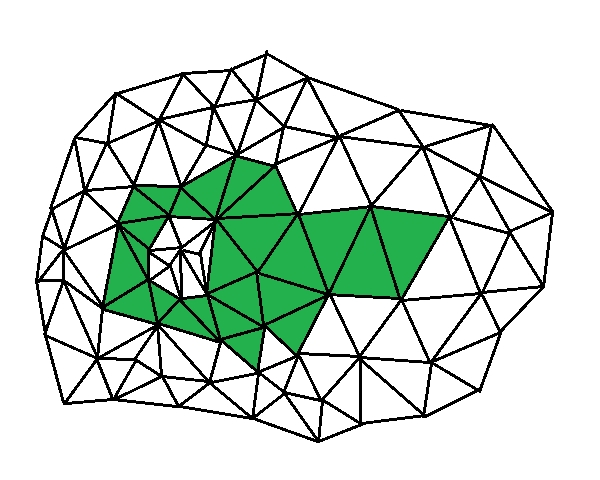
\includegraphics[scale=0.3]{Dila1.jpg}~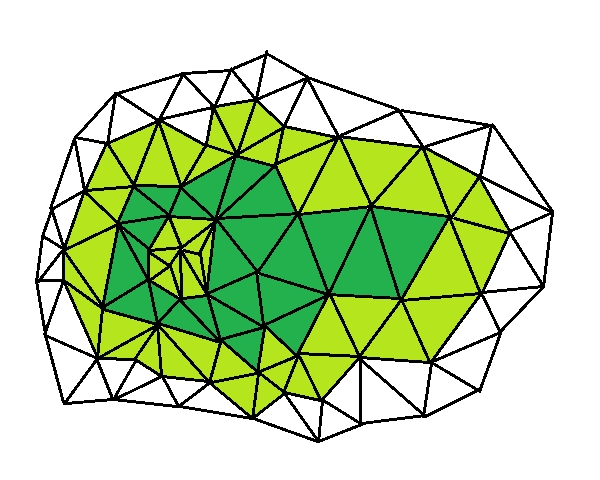
\includegraphics[scale=0.3]{Dila2.jpg}~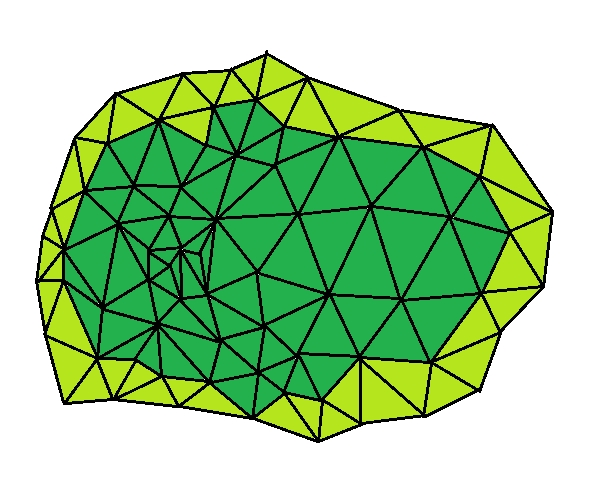
\includegraphics[scale=0.3]{Dila3.jpg}

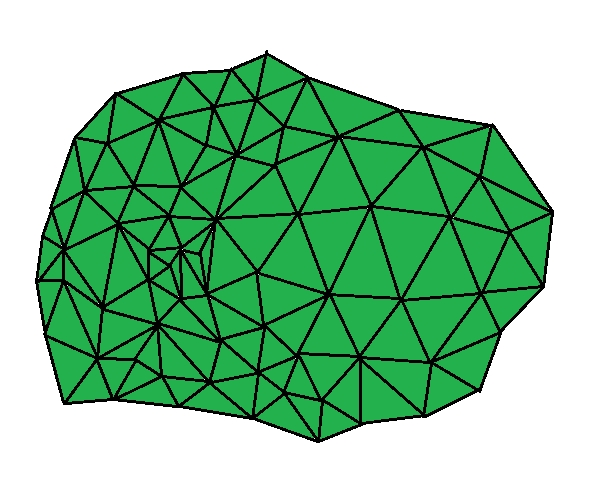
\includegraphics[scale=0.3]{Dila4.jpg}~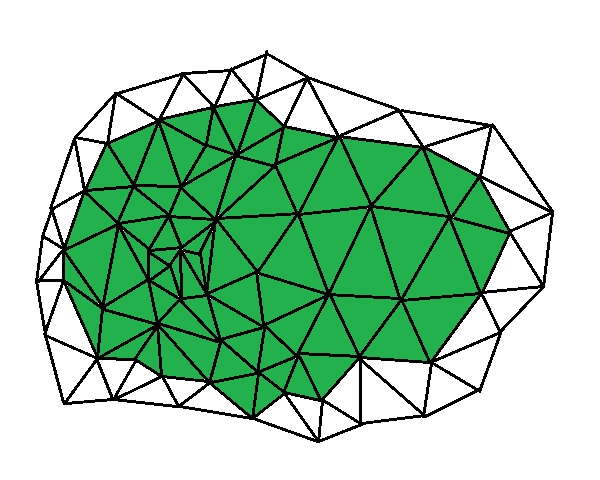
\includegraphics[scale=0.3]{Dila5.jpg}~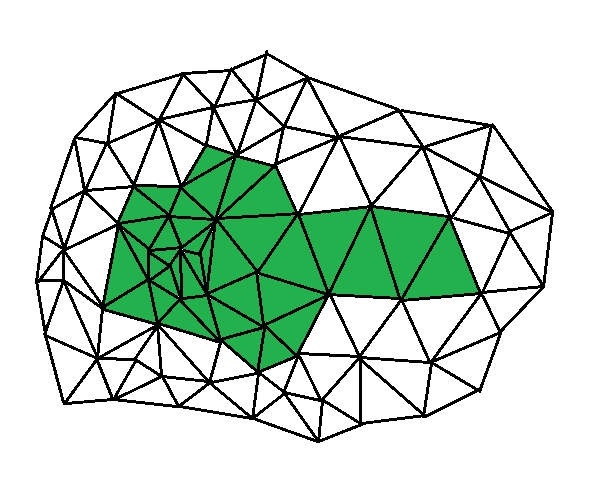
\includegraphics[scale=0.3]{Dila6.jpg}
\caption{\label{fig:DilEro} Étapes de dilatation/érosion}
\end{figure}

Les plans sont désormais détectés. La figure~\ref{fig:resultPlan} illustre le résultat de cette détection. Il faut maintenant modifier la géométrie du modèle pour faire apparaitre ces plans.

\begin{figure}[h]
\centering
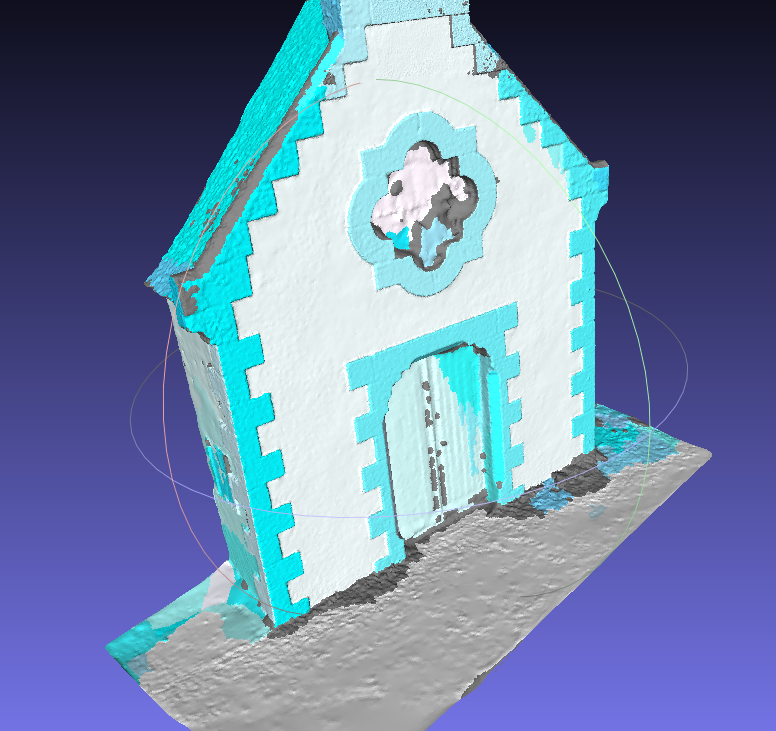
\includegraphics[scale=0.3]{Plan1.png} 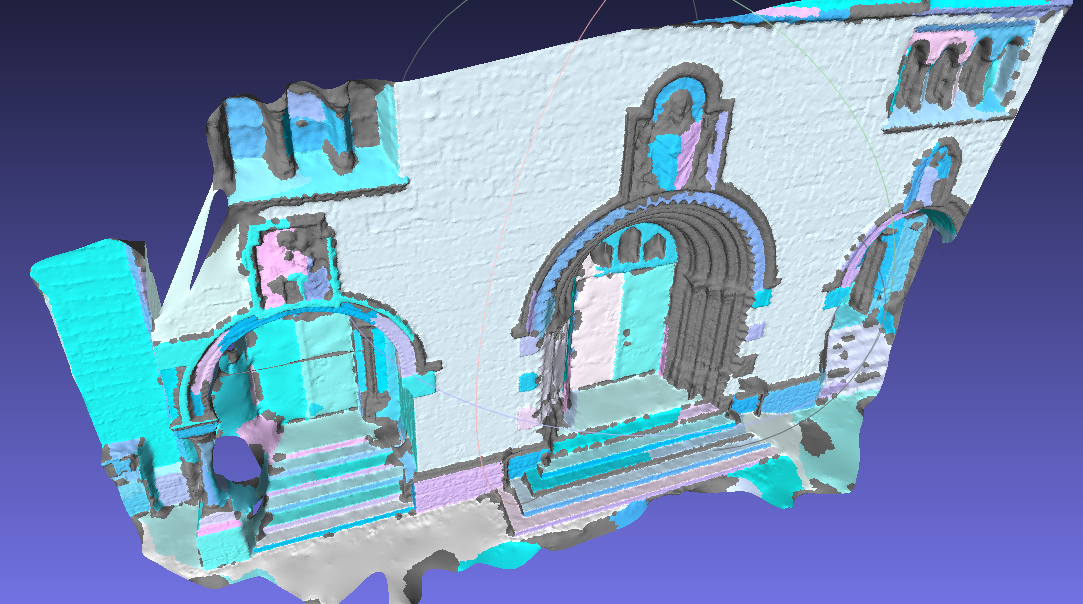
\includegraphics[scale=0.3]{Plan2.png} 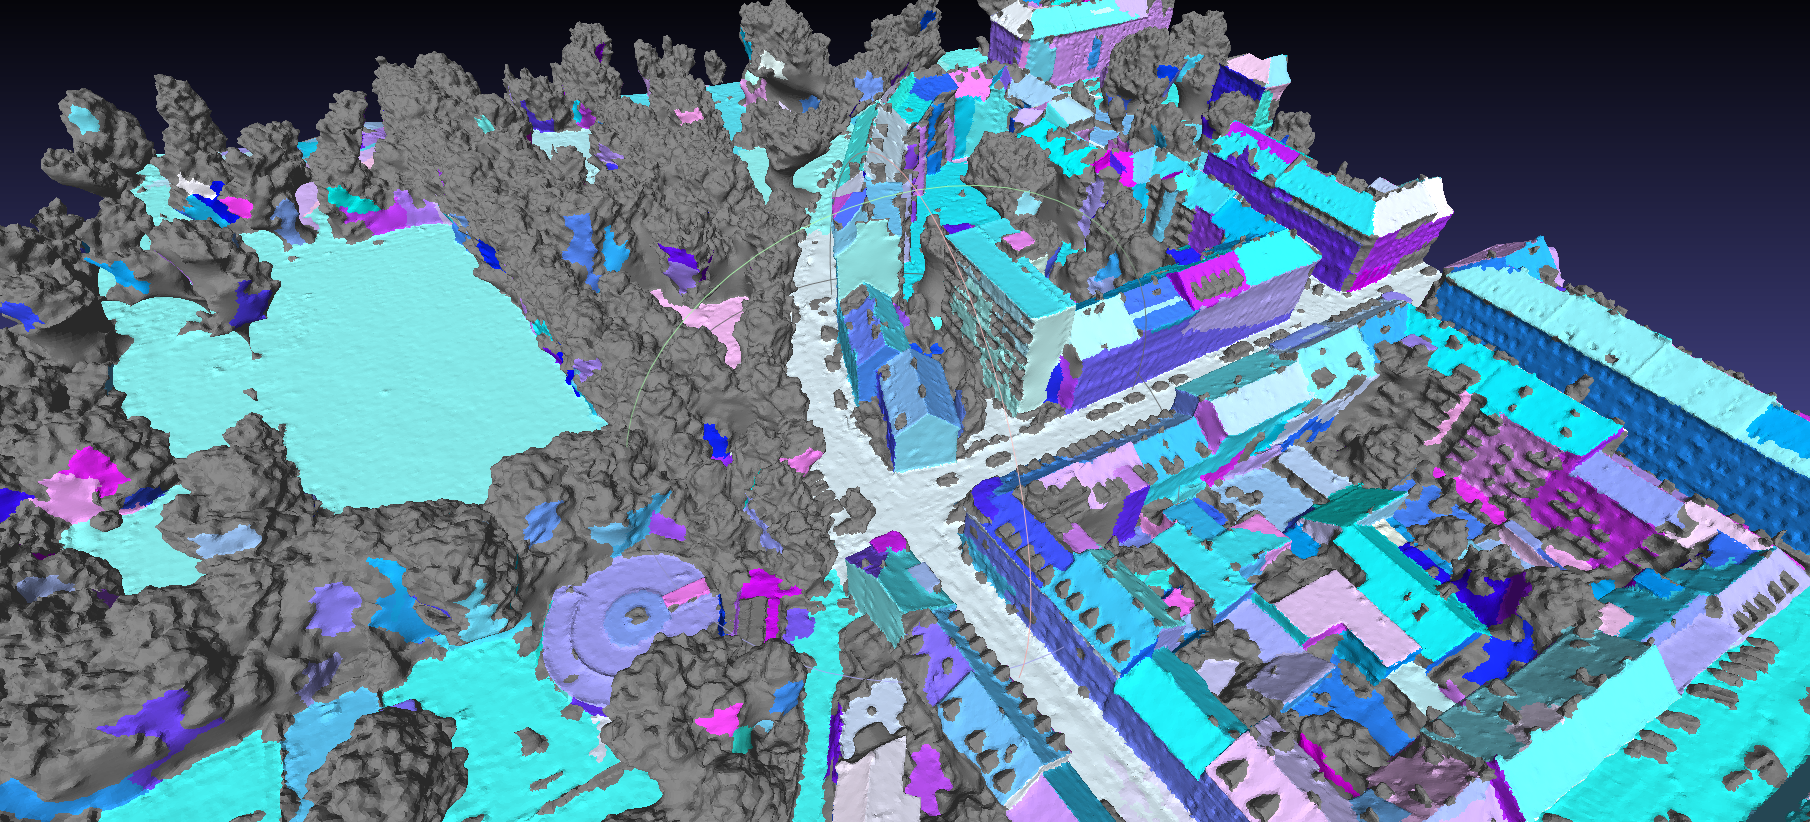
\includegraphics[scale=0.3]{Plan3.png}
\caption{\label{fig:resultPlan} Résultats de la détection de plan. Chaque plan est identifié par une couleur différente. Les zones en gris sombre sont les zones sans plan.}
\end{figure}

\section{Maillage}
\subsection{Problématique}
Maintenant que les plans sont détectés, il faut projeter les points sur ces plans, afin d'obtenir la géométrie voulue. Cependant, une simple projection directe des points sur les plans, les arêtes ou les coins engendre de mauvais résultats. La topologie du mesh est \textit{cassée} par la projection, comme en témoigne la figure~\ref{fig:probproj}.

\begin{figure}[h]
\centering
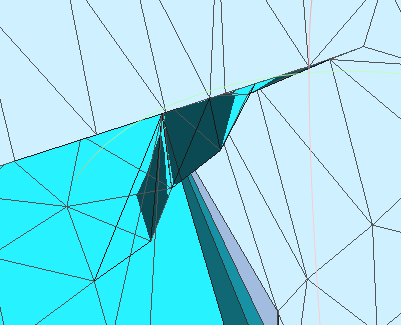
\includegraphics[scale=0.55]{prob1.png} 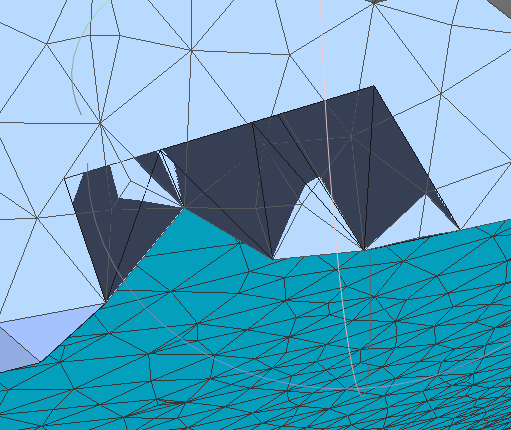
\includegraphics[scale=0.4]{prob2.png} 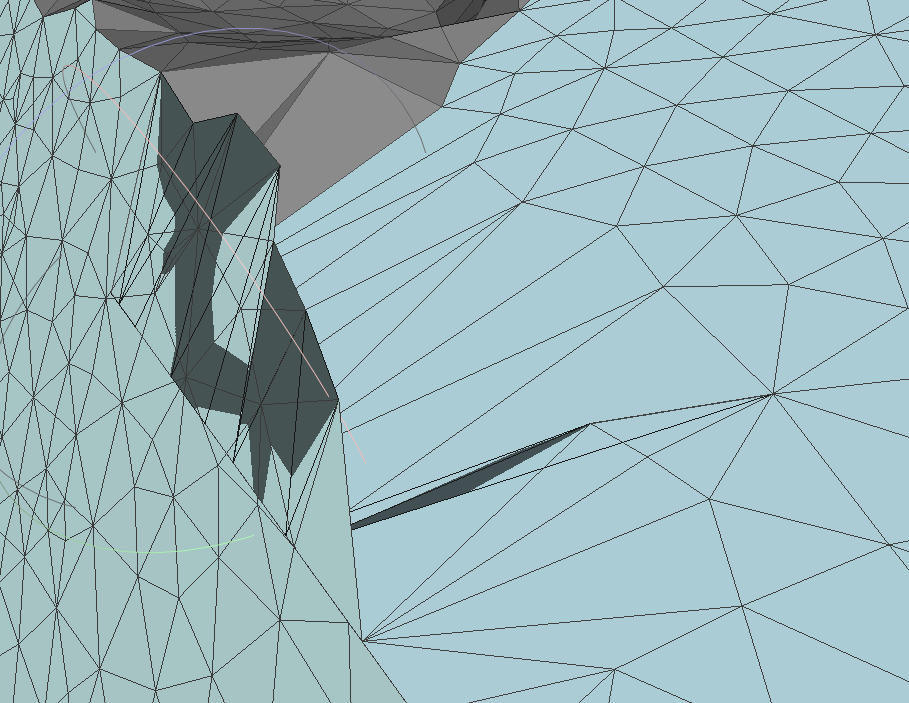
\includegraphics[scale=0.25]{prob3.png}
\caption{\label{fig:probproj} Problèmes de reprojection dues à la présence d'arêtes entre deux plans.}
\end{figure}

Il est donc nécessaire de traiter le nuage de points pour éviter ce genre d'erreur topologique et de recréer le maillage à partir du nuage de points et des informations précédemment calculées -- notamment la normale de chaque point.

\subsection{Traitement du nuage de points}
La première étape consiste à traiter correctement les points du mesh dans lequel les plans viennent d'être détectés. Pour cela, nous distinguons 4 types de points :
\begin{enumerate}
  \item Neutre -- aucune des facettes autour du point n'est attribuée à un plan ;
  \item Plan -- il y a au moins une facette attribuée à un plan autour du point, et il n'y a qu'un seul même plan parmi les facettes attribuées ;
  \item Arête -- il y a au moins une facette attribuée à un plan autour du point, et il n'y a que deux plans parmi les facettes attribuées ;
  \item Coin -- il y a au moins une facette attribuée à un plan autour du point, et il n'y a au moins trois plans parmi les facettes attribuées.
\end{enumerate}

\paragraph{Projection des points} Les points \textit{Neutre} ne sont pas déplacés. Les points \textit{Plan} sont projetés sur leur plan.

Pour les points \textit{Arête}, plusieurs cas se présentent. Dans un premier temps, on évalue sur les plans sont correctement orientés pour faire apparaître une arête. Cela se traduit par des normales ni trop proches ni trop opposées, puisque dans ces cas la projection risque d'être aberrante. Dans notre implémentation, le critère de bonne arête est le suivant
$$n_1\cdot n_2 < 0.9 \text{ et } n_1\cdot n_2 > -0.7$$
Si ce critère n'est pas satisfait, le point est déplacé sur le barycentre de ses projections sur chaque plan. Si le critère est satisfait, on crée un point correspondant à la projection du point traité orthogonalement sur l'arête formée par les deux plans. Si la distance entre les deux points est inférieure au seuil \texttt{Tolerance}, alors le point traité est déplacé sur la projection. Sinon, il est déplacé sur le barycentre de ses projections sur chaque plan -- si ce déplacement respecte aussi le seuil \texttt{Tolerance}.

Pour les points \textit{Coin}, il y a $N$ plans à traiter, $N \geq 3$. On commence par considérer chaque triplet de plans. Pour un triplet, on vérifie s'il est possible de projeter le point sur l'intersection des trois plans. Pour cela, on vérifie les critères suivants :
\begin{enumerate}
  \item $\vert n_1 \cdot n_2 \vert < 0.7$ ;
  \item $\vert n_1 \cdot n_3 \vert < 0.7$ ;
  \item $\vert n_2 \cdot n_3 \vert < 0.7$ ;
  \item $\vert (n_1 \wedge n_2) \cdot n_3 \vert > 0.3$ ;
  \item $\vert (n_1 \wedge n_3) \cdot n_2 \vert > 0.3$ ;
  \item $\vert (n_2 \wedge n_3) \cdot n_1 \vert > 0.3$.
\end{enumerate}
Les trois premiers critères servent à vérifier si chaque couple de plans forme une bonne arête. Les trois derniers servent à vérifier si nous sommes bien en présence d'un point d'intersection et non pas d'une droite : dans le cas extrême d'une intersection de plan formant une droite, les trois premiers critères sont vérifiés mais la projection ne peut pas être bonne. Les trois derniers paramètres évitent d'avoir des points qui sont projetés trop loin de leur position d'origine.

Si tous les critères sont vérifiés, on enregistre la position de l'intersection. Sinon on enregistre le barycentre des projections du point sur chaque plan. Une fois chaque triplet traité, on calcule le barycentre de chaque position obtenue et on déplace le point traité sur ce barycentre.

Cette étape permet de projeter correctement les points sur les plans. Cependant, ces précautions ne sont pas suffisantes pour respecter la topologie du maillage. Nous allons introduire et retirer des points afin de préparer une nouvelle triangulation du nuage de points, dans le but d'obtenir un maillage correct.

\paragraph{Échantillonage des arêtes} Nous introduisons des points le long des arêtes afin de faciliter le maillage le long de ces arêtes. Les arêtes sont détectées lors de la phase de projection. Lorsque un point de type \textit{Arête} ou \textit{Coin} est projeté sur l'arête ou l'intersection, alors ce point est ajouté à un objet \texttt{Ridge} correspondant à l'arête entre deux plans. Une fois tous les points ajoutés, on traite chaque arête. Les points des arêtes sont classés selon le vecteur directeur de l'arête. Cette dernière est ensuite séparée en \textit{chunks} : l'arête n'est pas forcément continue et un échantillonage naïf introduirait des défauts dans le modèle.

Une fois l'arête traitée, on échantillone chaque \textit{chunk}. La distance d'échantillonage est determinée par la distance moyenne entre chaque point de l'arête. Un point est ajouté sur l'arête toutes les demi-distances moyennes. Sachant que l'on garde les points déjà présents sur l'arête, le nombre de points est triplé.

\paragraph{Retrait des points incorrects} La projection des sommets a comme effet de replier la surface sur elle-même -- figure~\ref{fig:probproj} -- et ce malgré les précautions prises auparavant. Il convient donc de retirer les points qui posent problème.

La première étape consiste à repérer les sommets où la surface se replie. On cherche ainsi les points de type \textit{Plan}. Parmi ces points, on retient ceux qui ont au moins deux facettes dont la normale est inversée, c'est-à-dire tel que $n_{f_{1}} \cdot n_{f_{2}} = -1$ si les normales sont normalisées.

La seconde étape consiste à identifier les points qui se trouvent dans une zone où la surface est repliée. Pour cela, la méthode retenue car la plus efficace est de tester si un point \textit{tombe au milieu} d'une autre facette. Soit $a$, $b$ et $c$ les trois sommets d'une facette. Sachant que l'on travaille en 2D -- le plan est déjà projeté -- on identifie un point $p$ au milieu d'une facette de la manière suivante :
$$n_A = (b-a)\wedge(p-a) ; n_B = (c-b)\wedge(p-b) ; n_C = (a-c)\wedge(p-c)$$
$$\text{Si }n_A\cdot n_B > 0 \text{ et } n_A\cdot n_C > 0 \text{ et } n_B\cdot n_C > 0 \text{ alors le point est au milieu de la facette.}$$
Cette méthode reste lente car il faut vérifier pour chaque point d'un plan l'ensemble des facettes. Pour accélérer le traitement, cette phase est effectuée en parallèle et le choix des plans est affiné au fil des étapes. Ainsi, si aucun point d'un plan n'a été détecté dans la première étape, alors la seconde étape n'est pas appliquée à ce plan.

Les points identifiés lors de ces deux étapes sont retirés du nuage de points.

\paragraph{Informations de points} Pour permettre un meilleur maillage, nous avons besoin de certaines informations sur les points. Outre le type -- \textit{Neutre}, \textit{Plan}, \textit{Arête} ou \textit{Coin} -- nous avons aussi besoin de l'échantillonage et de la normale. L'échantillonage correspond à la longueur de la plus grande arête reliée au point. Dans le cas de points rajoutés, l'échantillonage est fixé à la distance moyenne entre les points de l'arête. La normale est calculée comme étant la moyenne des normales des facettes entourant le point. Pour les points rajoutés, la normale est la moyenne des deux normales des plans formant l'arête.\newline

Désormais, nous avons tous les élèments en main pour créer le nouveau maillage du modèle.

\subsection{Maillage du nuage de points}
Pour mailler ce nuage de points, nous reprenons les méthodes utilisées par \textit{Smart3DCapture}. Le maillage du nuage de points est largement inspiré de \cite{maillage1}. Afin de s'adapter à la spécificité de notre modèle avec plans, notre méthode s'inspire aussi de \cite{maillage2}.

\cite{maillage1} présente une méthode pour obtenir une surface à partir d'un nuage de point et d'informations de visibilités. On effectue d'abord une triangulation 3D du nuage de points. Ensuite, chaque tétraèdre -- appelé aussi cellule -- est traité à l'aide des informations de visibilités. Le but est de déterminer si la cellule est à l'intérieur ou à l'extérieur de la surface. Pour chaque cellule, des scores sont calculés. Des coûts sont aussi calculés entre les faces de chaque cellule. La surface est ensuite extraite à l'aide d'un \textit{graphcut}. Le \textit{graphcut} est un algorithme de coupe minimale. Le but est d'obtenir la surface qui sépare les cellules en deux parties distinctes avec un score minimal. Des dispositions sont prises afin d'éviter la solution triviale de la surface vide.

Nous réutilisons cette technique du \textit{graphcut} mais nous calculons de nouveaux coûts, plus adaptés à notre mesh.

\paragraph{Coût des cellules} Le coût des cellules doit refléter la propriété de la position de la cellule par rapport à la surface, autrement dit la présence de la cellule à l'intérieur ou à l'extérieur de la surface. Pour évaluer cette propriété, nous nous basons sur les normales de chaque point. De manière intuitive, si les quatre normales d'une cellule pointent vers l'intérieur de la cellule, c'est que cette dernière est à l'extérieur de la surface. De la même façon, si les quatre normales pointent vers l'extérieur, la cellule se trouve à l'intérieur de la surface -- figure~\ref{fig:inout}.

XXX FIGURE IN OUT

Le score de la cellule est calculé à l'aide de son barycentre $b$. Pour chaque sommet -- $s_1, s_2, s_3, s_4$ -- on calcule le produit scalaire $\dfrac{n_i\cdot(b-s_i)}{\Vert b-s_i\Vert}$ et on l'ajoute au score. Si $\dfrac{n_i\cdot(b-s_i)}{\Vert b-s_i\Vert} > 0.3$, on ajoute $1$ au score. Si $\dfrac{n_i\cdot(b-s_i)}{\Vert b-s_i\Vert} < -0.3$, on retranche $1$ au score. Les cellules à l'intérieur ont un score négatif et celles à l'extérieur un score positif. Le seuil de $\pm 0.3$ permet de favoriser les normales qui caractérisent vraiment la cellule par rapport aux normales plus ambiguës.

\paragraph{Coût des facettes} \cite{maillage2} introduit un coût pour les facettes prenant en compte les plans détectés. Le principe générale est d'empêcher le \textit{graphcut} de passer par une facette qui serait incohérente vis-à-vis de la géométrie détectée. Plusieurs catégories de facettes sont introduites :
\begin{enumerate}
  \item Facette dite \textit{Free-form coherent}. Ce sont les facettes avec 0, 1 ou 2 points de type \textit{Plan} appartenant au même plan.
  \item Facette dite \textit{Structurally coherent}. Ce sont les facettes avec :
  \begin{itemize}
    \item 3 points de type \textit{Plan} appartenant au même plan ;
    \item 2 points de type \textit{Plan} reliés au plan $i$ et 1 point de type \textit{Arète} relié aux plans $i$ et $j$ ;
    \item 2 points de type \textit{Arête} reliés aux plans $i$ et $j$ et 1un point de type \textit{Plan} relié au plan $i$ ;
    \item 2 points de type \textit{Plan} reliés au plan $i$ et un point de type \textit{Coin} relié aux plans $i$, $j$ et $k$ ;
    \item 2 points de type \textit{Arête} reliés respectivement aux plans $i$ et $j$ et aux plans $j$ et $k$ et 1 point de type \textit{Coin} relié aux plans $i$, $j$ et $k$ ;
    \item 1 point de type \textit{Plan} relié au plan $i$, 1 point de type \textit{Arête} relié aux plans $i$ et $j$, 1 point de type \textit{Coin} relié aux plans $i$, $j$ et $k$ ;
  \end{itemize}
  \item Facette dite non-cohérente.
\end{enumerate}

La figure~\ref{fig:coherence} illustre ces catégories.

\begin{figure}[h]
\centering
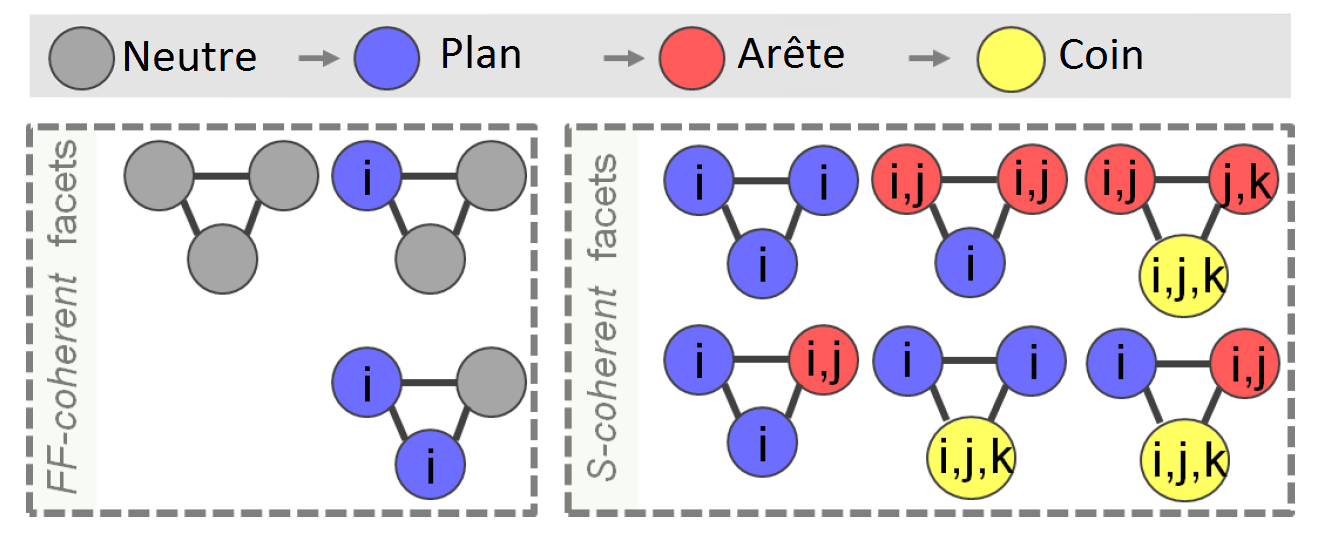
\includegraphics[scale=0.4]{coherent.png}
\caption{\label{fig:coherence} Les facettes \textit{Free-form coherent} et \textit{Structurally coherent}.}
\end{figure}

Dans notre implémentation, nous avons rajouté un septième type de facette \textit{Structurally coherent}. Il s'agit d'une facette composée de 2 points de type \textit{Arête} reliés aux plans $i$ et $j$ et d'un point de type \textit{Arête} reliés aux plans $j$ et $k$. Ce type de facette est nécessaire pour mailler correctement un plan qui se termine en pointe fine.

Selon la catégorie de la facette, le coût ne sera pas le même. Les facettes \textit{Structurally coherent} ont un coût nul. Les facettes \textit{Free-form coherent} entraînent un coût léger, alors que les facettes \textit{not coherent} entraînent un coût élevé. L'objectif est d'empécher la surface de passer par ces facettes. Si le coût est trop élevé, la surface ne passera pas par cette facette.

Le coût des cellules permet surtout d'obtenir une surface similaire à celle d'origine dans les zones non planaires. La figure~\ref{fig:comparo} illustre la faible différence entre le maillage d'origine et le maillage recalulé.

\begin{figure}[h]
\centering
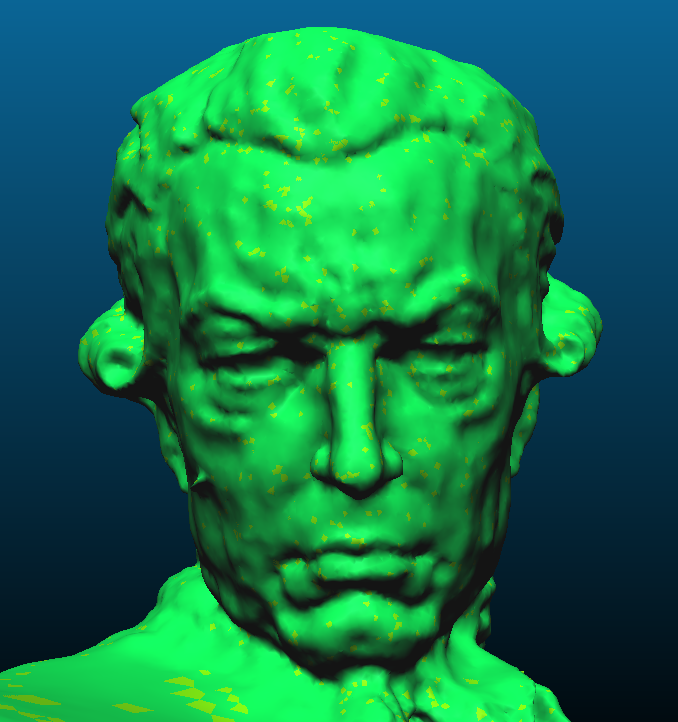
\includegraphics[scale=0.4]{Comparo2.png} 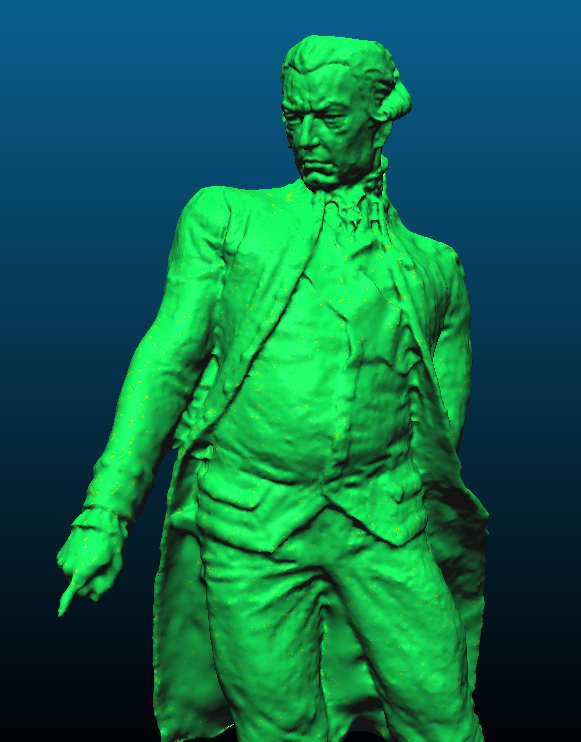
\includegraphics[scale=0.4]{Comparo3.png}
\caption{\label{fig:comparo} Les triangles en vert atteste d'un décalage nul, les triangles en jaune d'un décalage de moins de 1\%.}
\end{figure}

Le coût des facettes permet d'éviter une mauvaise triangulation, notamment lorsque deux plans se trouvent côte à côte. La figure~\ref{fig:avap} montre la différence entre l'ancien maillage et le nouveau maillage.

À noter que lors de l'extraction de la surface, on obtient de larges facettes incohérentes avec la scène. Avant de les traiter, on se base sur l'échantillonage de chaque point. Si un point est relié à une arête dont la longueur est largement supérieure à la distance d'échantillonage du point, alors la facette est rétirée. Cette étape de filtrage est surtout utile au niveau des bords du modèle.

Le maillage est désormais cohérent avec la scène. Il est maintenant nécessaire de le simplifier afin de réduire le poids du modèle.

\begin{figure}[h]
\centering
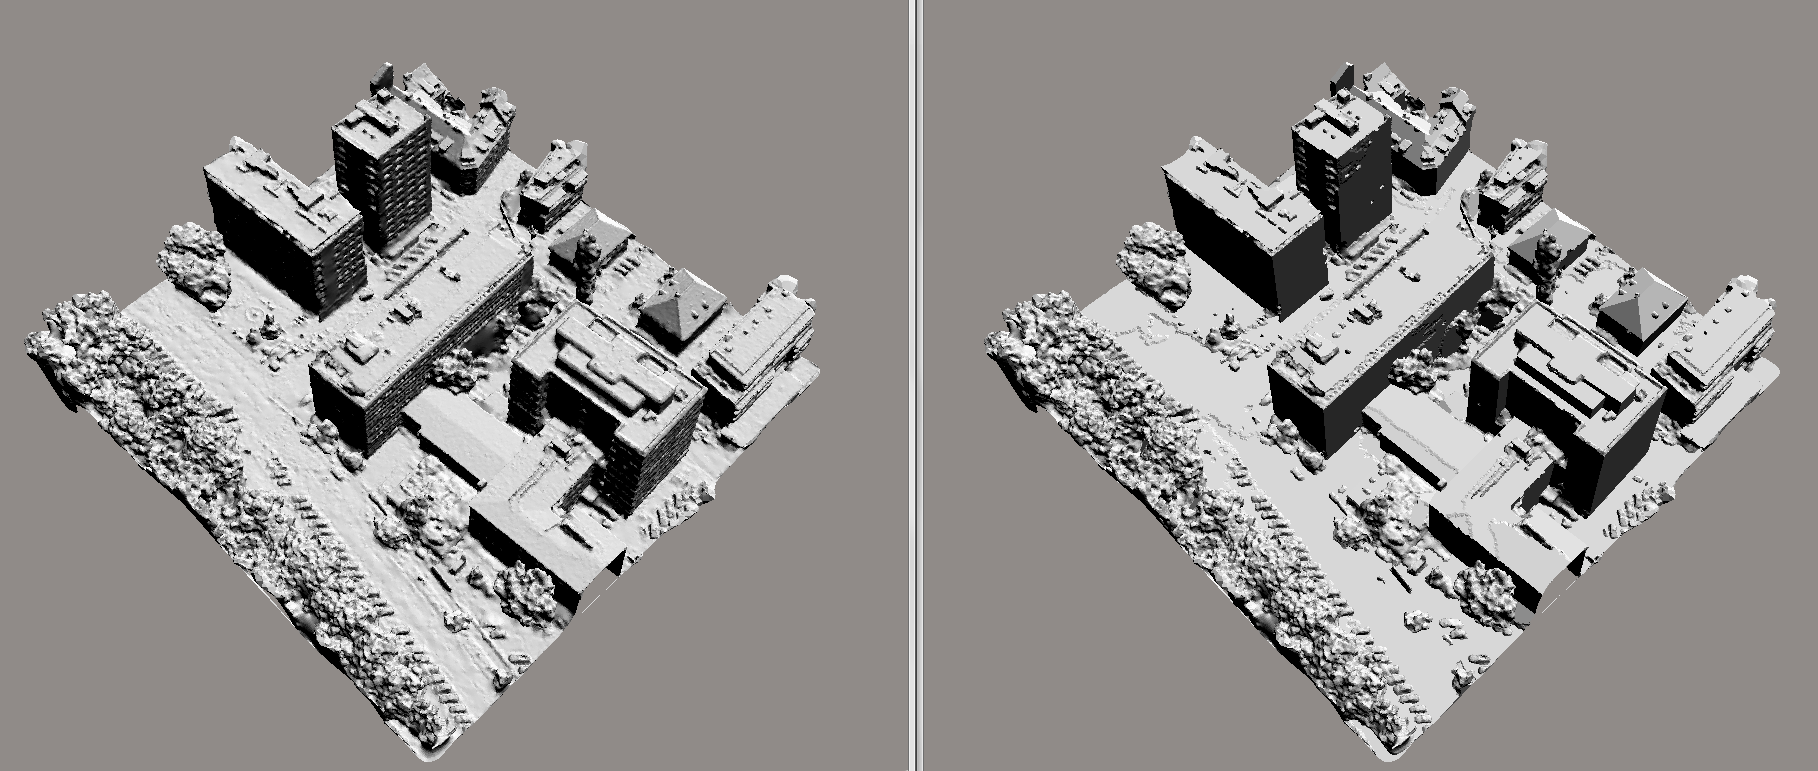
\includegraphics[scale=0.35]{Comparo4.png} 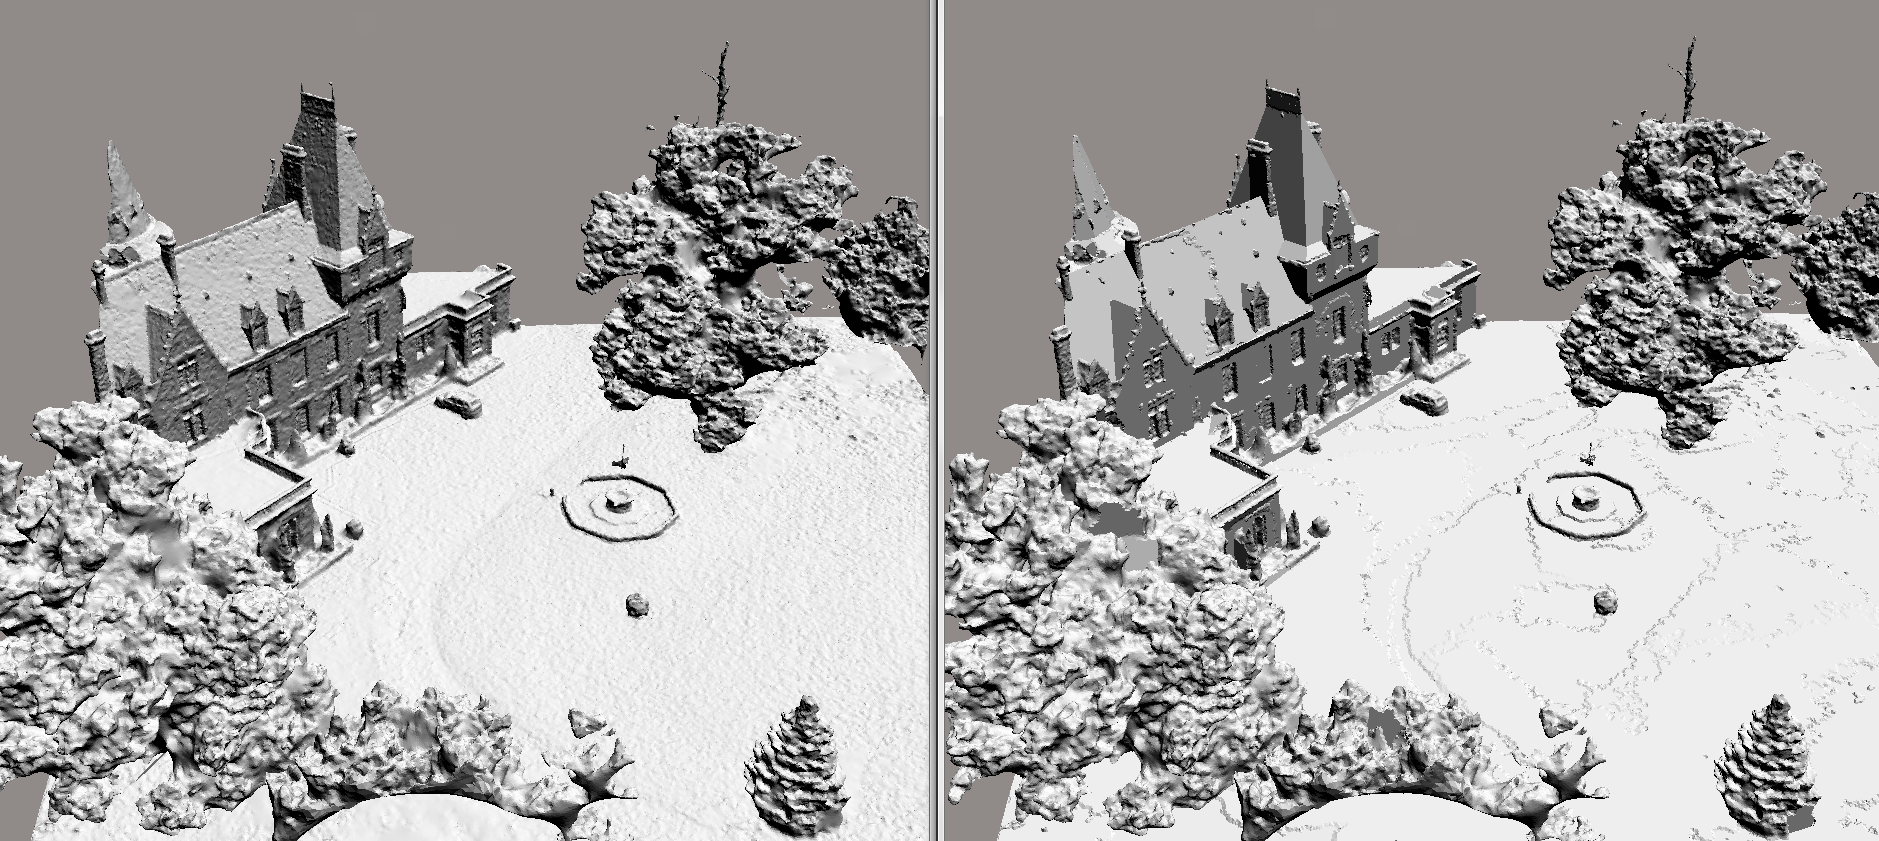
\includegraphics[scale=0.34]{Comparo5.png} 
\caption{\label{fig:avap} À gauche, l'ancien maillage. À droite, le nouveau maillage.}
\end{figure}

\section{Simplification}
\subsection{Problématique}
Les modèles obtenus après le remaillage sont extrêmement détaillés, autant dans les parties planes que dans les parties non-planes. Il est nécessaire que notre algorithme de simplification puisse s'adapter autant aux parties planes qu'aux parties présentant des détails fins. Il faut aussi que cet algorithme conserve la planarité des plans détectés.

\subsection{Simplification existante et limitations}
Actuellement, \textit{Smart3DCapture} utilise un algorithme de simplification basé sur un mécanisme d'\textit{edge collapse}. Cet algorithme provient de la librairie \texttt{CGAL} et son implémentation provient majoritairement de \cite{simp1, simp2}. Le principe de l'algorithme est de fusionner certains sommets entre eux pour réduire le nombre de facettes tout en conservant au mieux la géométrie du modèle.

Pour chaque sommet, une quadrique est calculée. La quadrique correspond à l'ensemble des 10 paramètres décrivant la surface localement autour du point. Pour chaque arête, on calcule le point qui minimise l'erreur de quadrique lorsque l'arête est supprimée ainsi que le coût de cette erreur. Si le déplacement du point est trop important, on utilise plutôt le placement de Lindstrom-Turk \cite{simp2}. Ensuite, on traite les arêtes par ordre croissant de coût : on simplifiera d'abord les zones où le coût de déplacement est faible. La simplification s'arrête une fois que la somme des erreurs dépasse un certain seuil.

\begin{figure}[h]
\centering
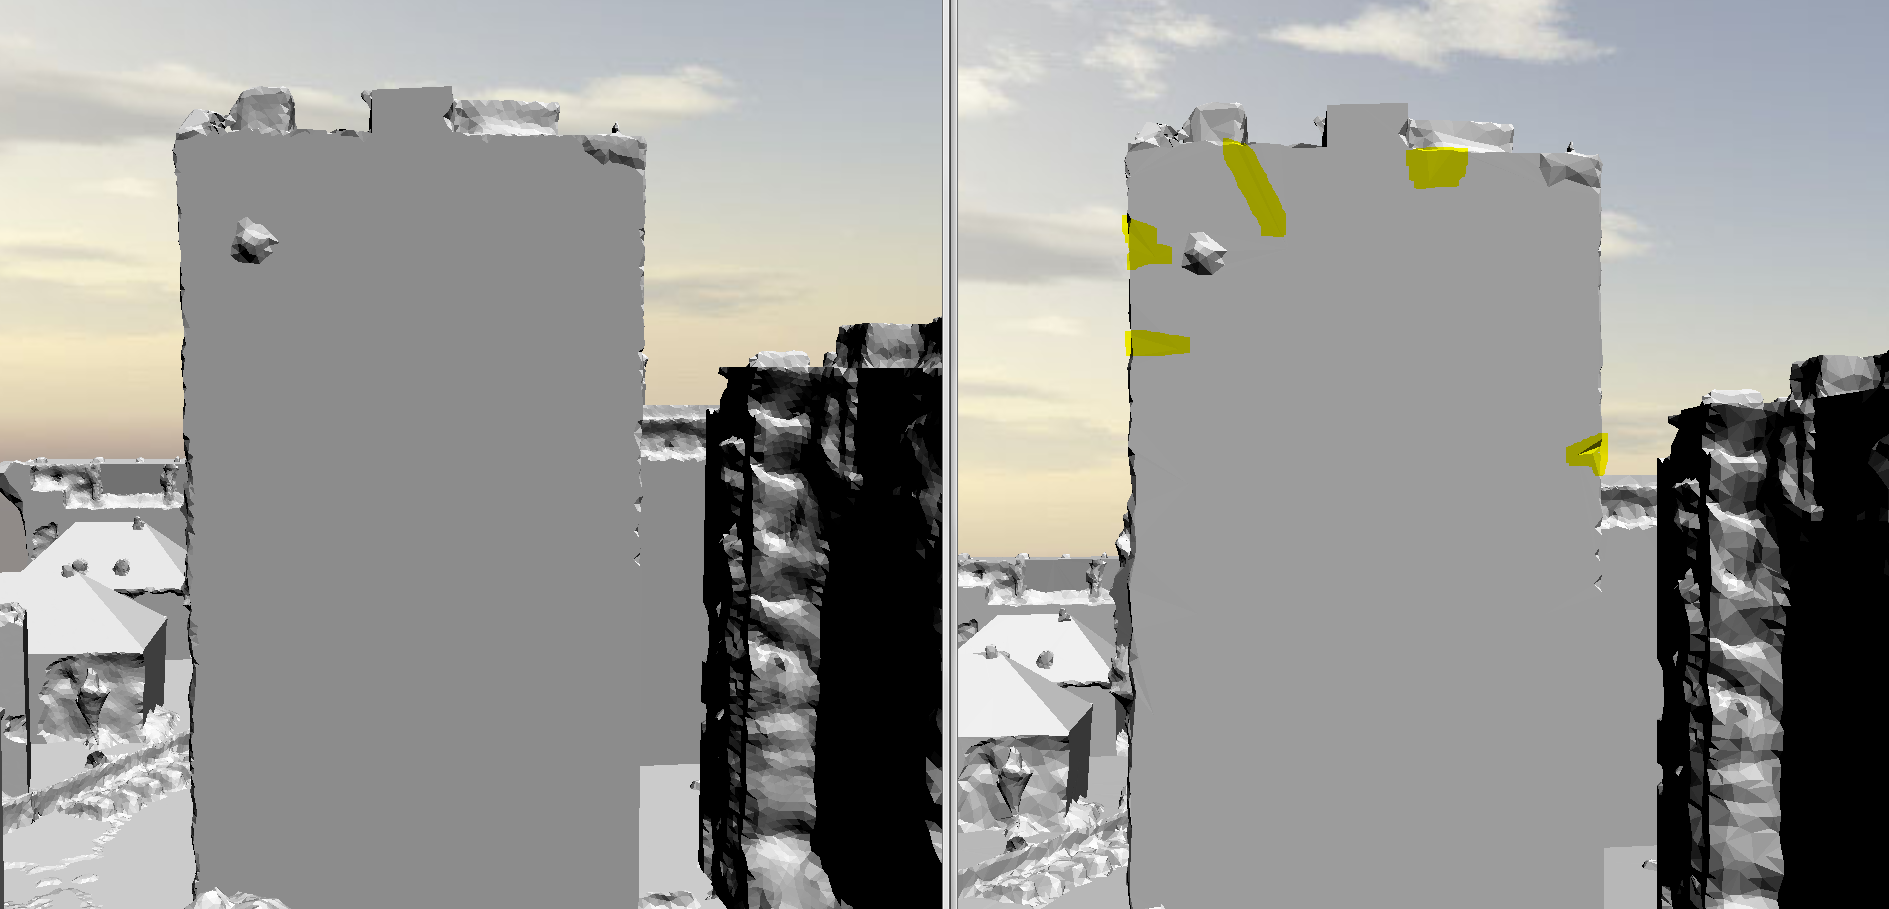
\includegraphics[scale=0.33]{Simpli1.png}
\caption{\label{fig:simpl1} À gauche, le maillage non simplifié. À droite, le maillage simplifié via la méthode classique.}
\end{figure}

La figure~\ref{fig:simpl1} expose le problème de l'algorithme de simplification actuel. On remarque que sur les bords du plan, le maillage simplifié n'est pas tout à fait plan. De plus, la simplification est parfois trop importante -- cf l'entaille sur le bord droit de l'immeuble.

\subsection{Modifications}
Nous avons modifié l'algorithme de simplification pour tenir compte des spécificités de notre maillage.

La première modification concerne le placement. Lorsque le placement optimal est calculé, nous voulons être certain que le placement est cohérent par rapport au maillage initial. Pour cela, le point obtenu via le placement optimal est ensuite projeté sur le plan, l'arête ou le coin associé. Cette nouvelle projection nous permet d'être certain que la géométrie des plans et des arêtes est respectée.

La seconde modification concerne l'estimation du coût de déplacement. Lorsque l'un des points fusionnés est intégralement entouré de facettes assignées à un plan, alors on estime que le coût du déplacement doit être nul. Si le coût n'est pas nul, alors on modifie ce coût à un coût infini. Cela signifie que nous voulons que la simplification n'entraîne aucune perte de précision.

Un coût particulier est aussi créé pour les bordures du maillage qui sont planes. En effet, à cet endroit le mécanisme d'\textit{edge collapse} n'entraîne aucun coût puisque le point reste dans le plan. Mais le point est tout de même décalé au milieu de l'arête : la simplification ronge ainsi les bords du maillage plan. our éviter ce phénomène, on introduit un coût de distance : dans le cas d'une arête en bordure de maillage, si la distance entre le nouveau et l'ancien point est supérieure à un seuil, alors on attribue un coût infini à la suppression de l'arête.

\begin{figure}[h]
\centering
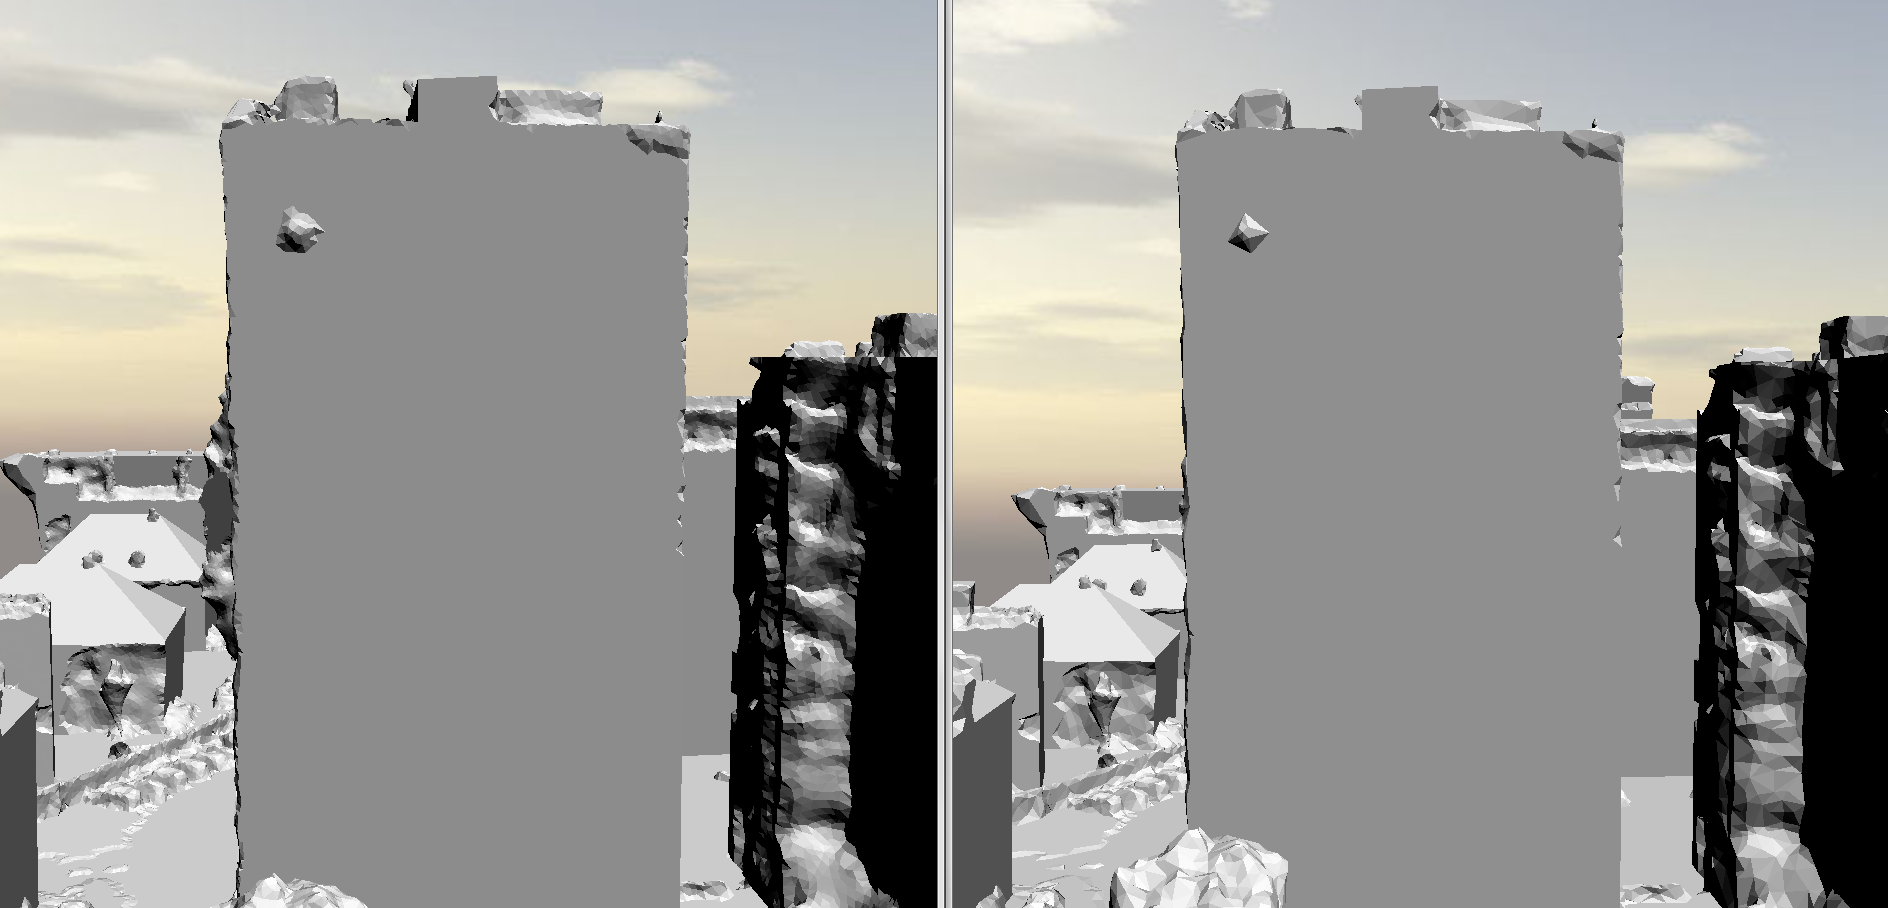
\includegraphics[scale=0.33]{Simpli2.png}
\caption{\label{fig:simpl2} À gauche, le maillage non simplifié. À droite, le maillage simplifié via la méthode modifiée.}
\end{figure}

La figure~\ref{fig:simpl2} montre l'amélioration du maillage à l'aide de notre méthode. La modification du placement donne de plus de meilleurs résultats sur les bordures des plans.

\section{Résultats}
\subsection{Niveaux de simplification}
\subsection{Temps d'éxécution}
\subsection{Gain de place}
\subsection{Problèmes existants}

\newpage
\section*{Conclusion}
\addcontentsline{toc}{section}{Conclusion}

\newpage
\bibliographystyle{alpha}
\bibliography{biblio}
\addcontentsline{toc}{section}{References}
\newpage
\appendix
\section{Calcul}
Test popopopopop
\end{document}